Im ersten Aufgabenteil wird eine Referenzspannung von $U_\text{ref}=6.56 \si{\volt}$
eingestellt. Die Frequenz wird hierbei manuell eingestellt und die Spannungsamplituden
$U_\text{SS}$ werden peak-to-peak gemessen.


\begin{table}[!h]
  \centering
  \begin{subtable}{0.3\textwidth}
    \begin{tabular}{S[table-format=4.0]S}
      \toprule
      {$\varphi$} &
      {$U_\text{SS} \,/\, \si{\volt}$} \\
      \midrule
      15\si{\degree} & 0.82  \\
      45\si{\degree} & 0.81 \\
      105\si{\degree} & 0.46  \\
      165\si{\degree} & 0.88 \\
      225\si{\degree} & 0.82  \\
      330\si{\degree}  & 0.83  \\
      \bottomrule
    \end{tabular}
    \caption{ohne Tiefpass}
    \label{tab:a}
  \end{subtable}
  \quad
  \begin{subtable}{0.3\textwidth}
    \begin{tabular}{S[table-format=4.0]SS}
      \toprule
      {$\varphi$} &
      {$U_\text{max} \,/\, \si{\volt}\cdot10^{-3}$} &
      {$U_\text{out} \,/\, \si{\volt}\cdot10^{-3}$} \\
      \midrule
      0\si{\degree}    &    -5     &     -3.18 \\
     15\si{\degree}    &     5     &      3.07 \\
     30\si{\degree}    &    25     &     13.78 \\
     45\si{\degree}    &    45     &     20.27 \\
     90\si{\degree}    &    80     &      0.00 \\
    120\si{\degree}    &    78     &     24.83 \\
    135\si{\degree}    &    65     &    -29.26 \\
    165\si{\degree}    &    20     &    -12.30 \\
    180\si{\degree}    &    5      &     -3.18 \\
    210\si{\degree}    &    -25    &     13.78 \\
    225\si{\degree}    &    -53    &     23.86 \\
    255\si{\degree}    &    -80    &     13.18 \\
    \bottomrule
    \end{tabular}
    \caption{mit Tiefpass}
    \label{tab:b}
  \end{subtable}
  \caption{Messwerte ohne Rauschen}
  \quad
  \hfill
\end{table}


\begin{table}[!h]
  \centering
\begin{subtable}{0.3\textwidth}
  \begin{tabular}{S[table-format=4.0]S}
    \toprule
    {$\varphi$} &
    {$U_\text{SS} \,/\, \si{\milli\volt}$} \\
    \midrule
    0\si{\degree}   & 88.0  \\
    120\si{\degree} & 56.8  \\
    165\si{\degree} & 92.0  \\
    240\si{\degree} & 67.2  \\
    270\si{\degree} & 48.8  \\
    315\si{\degree} & 70.4  \\
    \bottomrule
  \end{tabular}
  \caption{ohne Tiefpass}
  \label{tab:c}
\end{subtable}
\quad
\begin{subtable}{0.3\textwidth}
  \begin{tabular}{S[table-format=4.0]SS}
    \toprule
    {$\varphi$} &
    {$U_\text{max} \,/\, \si{\volt}\cdot10^{-4}$} &
    {$U_\text{out} \,/\, \si{\volt}\cdot10^{-4}$} \\
    \midrule
    0   \si{\degree}  &    0     &      0.00 \\
   15   \si{\degree}  &    5     &      3.07 \\
   30   \si{\degree}  &    16    &      8.82 \\
   45   \si{\degree}  &    35    &     15.76 \\
   90   \si{\degree}  &    50    &      0.00 \\
  120   \si{\degree}  &    46    &    -14.64 \\
  135   \si{\degree}  &    38    &    -17.11 \\
  165   \si{\degree}  &    10    &     -6.15 \\
  180   \si{\degree}  &    1     &     -0.64 \\
  210   \si{\degree}  &    -20   &     11.03 \\
  225   \si{\degree}  &    -35   &     15.76 \\
  255   \si{\degree}  &    -50   &      8.24 \\
    \bottomrule
  \end{tabular}
  \caption{mit Tiefpass}
  \label{tab:d}
\end{subtable}
\caption{Messwerte mit Rauschen, Signal Attenuator = 1,
        Noise Amplitude = 1$\times 10^{-3}$.}
\quad
\hfill
\end{table}

Die Werte für $U_{out}$ lassen sich mit Hilfe der Formel \eqref{eqn:out} berechnen.\\

\begin{figure}[!h]
\begin{minipage}[t]{0.3\textwidth}
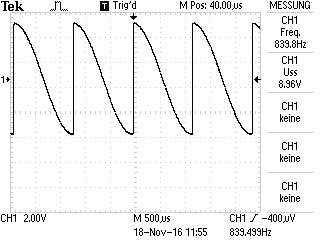
\includegraphics[width=\textwidth]{Bilder/15.jpg}
\caption{$\varphi = 15\si{\degree}$}
\label{fig:1}
\end{minipage}
\hspace{10pt}
\vspace{5pt}
\begin{minipage}[t]{0.3\textwidth}
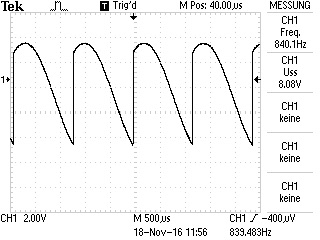
\includegraphics[width=\textwidth]{Bilder/45.jpg}
\caption{$\varphi = 45\si{\degree}$}
\label{fig:2}
\end{minipage}
\hspace{10pt}
\vspace{5pt}
\begin{minipage}[t]{0.3\textwidth}
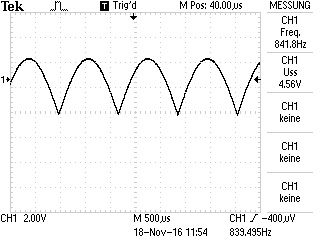
\includegraphics[width=\textwidth]{Bilder/105.jpg}
\caption{$\varphi = 105\si{\degree}$}
\label{fig:3}
\end{minipage}
\hspace{10pt}
\vspace{5pt}
\begin{minipage}[t]{0.3\textwidth}
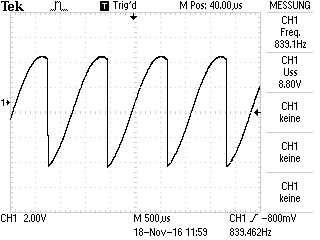
\includegraphics[width=\textwidth]{Bilder/165.jpg}
\caption{$\varphi = 165\si{\degree}$}
\label{fig:4}
\end{minipage}
\hspace{12pt}
\vspace{5pt}
\begin{minipage}[t]{0.3\textwidth}
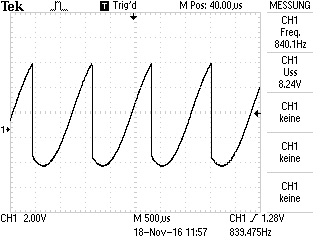
\includegraphics[width=\textwidth]{Bilder/225.jpg}
\caption{$\varphi = 225\si{\degree}$}
\label{fig:5}
\end{minipage}
\hspace{12pt}
\vspace{5pt}
\begin{minipage}[t]{0.3\textwidth}
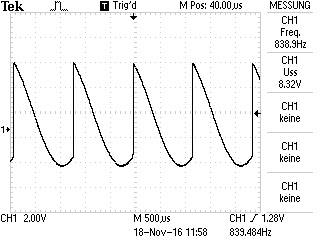
\includegraphics[width=\textwidth]{Bilder/330.jpg}
\caption{$\varphi = 330\si{\degree}$}
\label{fig:6}
\end{minipage}
\hspace{12pt}
\vspace{5pt}
\end{figure}

In den Abbildungen \eqref{fig:1} bis \eqref{fig:6} sind die Spannungskurven für unterschiedliche Phasen
zu sehen. Hierbei wurde weder der Tiefpassfilter noch der Rausch-Generator eingeschaltet. \\
Die Spannungswerte sind in (\ref{tab:a}) zu finden. \\

\newpage

\begin{figure}[!h]
\begin{minipage}[t]{0.3\textwidth}
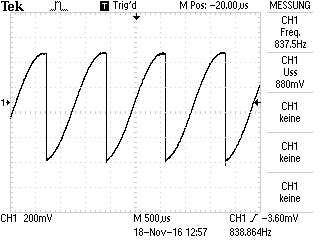
\includegraphics[width=\textwidth]{Bilder/Rausch0.jpg}
\caption{$\varphi = 0\si{\degree}$}
\label{fig:7}
\end{minipage}
\hspace{10pt}
\vspace{5pt}
\begin{minipage}[t]{0.3\textwidth}
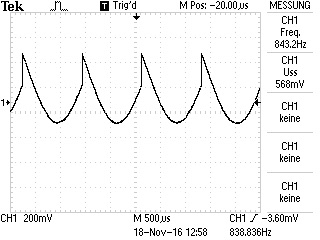
\includegraphics[width=\textwidth]{Bilder/Rausch120.jpg}
\caption{$\varphi = 45\si{\degree}$}
\label{fig:8}
\end{minipage}
\hspace{10pt}
\vspace{5pt}
\begin{minipage}[t]{0.3\textwidth}
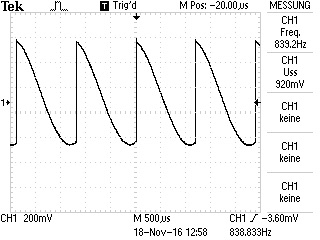
\includegraphics[width=\textwidth]{Bilder/Rausch165.jpg}
\caption{$\varphi = 90\si{\degree}$}
\label{fig:9}
\end{minipage}
\hspace{10pt}
\vspace{5pt}
\begin{minipage}[t]{0.3\textwidth}
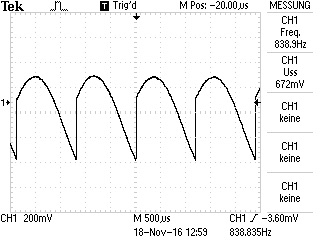
\includegraphics[width=\textwidth]{Bilder/Rausch240.jpg}
\caption{$\varphi = 135\si{\degree}$}
\label{fig:10}
\end{minipage}
\hspace{12pt}
\vspace{5pt}
\begin{minipage}[t]{0.3\textwidth}
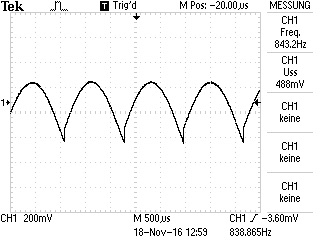
\includegraphics[width=\textwidth]{Bilder/Rausch270.jpg}
\caption{$\varphi = 180\si{\degree}$}
\label{fig:11}
\end{minipage}
\hspace{12pt}
\vspace{5pt}
\begin{minipage}[t]{0.3\textwidth}
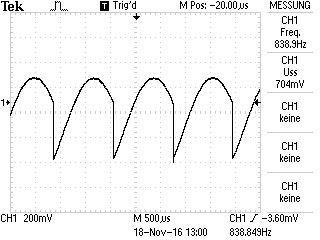
\includegraphics[width=\textwidth]{Bilder/Rausch315.jpg}
\caption{$\varphi = 180\si{\degree}$}
\label{fig:12}
\end{minipage}
\hspace{12pt}
\vspace{5pt}
\end{figure}

In den Abbildungen \eqref{fig:7}) bis \eqref{fig:12} sind die Spannungskurven mit
eingeschaltetem Rausch-Generator zu sehen. Der Tiefpassfilter ist weiterhin ausgeschaltet. \\
Die Spannungswerte sind in (\ref{tab:c}) zu finden. \\

\newpage

Im zweiten Teil der Auswertung wird die Abhängigkeit der Ausgangsspannung zur Phasenverschiebung
betrachtet. Hier wird sowohl mit, als auch ohne Rausch-Generator gemessen. Zur besseren
Darstellung wird $\varphi$ gegen $U_{out}$ geplottet. Diese Werte sind in Tabelle (\ref{tab:b}) einzusehen.

\begin{figure}[H]
  \centering
  \includegraphics[width=1.0\textwidth]{Bilder/phi.pdf}
  \caption{U$_{out}$ in Abhängigkeit von $\varphi$.}
  \label{fig:Uout}
\end{figure}

Die Funktionen in Grafik (\ref{fig:Uout}) lassen einen cosinusförmigen Verlauf erkennen. \\

\newpage


Im letzten Teil der Auswertung wurde untersucht, bei welcher maximalen Entfernung $r$
eine Photodiode keinen Lichtimpuls einer LED mehr aufnimmt. Dabei wird die eingehende Spannung $U$
gegen den Abstand $r$ geplottet.
\begin{figure}[H]
  \centering
  \includegraphics[width=\textwidth]{Bilder/Plot_Photodiode.pdf}
  \caption{U in Abhängigkeit von r}
  \label{fig:led}
\end{figure}

In Grafik (\ref{fig:led}) ist zu erkennen, dass die Spannung exponentiell zum Abstand
abnimmt. Daraus folgt:

\begin{equation*}
  U \propto \frac{1}{r^2}
\end{equation*}
\\
Nun wird die Ausgangsspannung gegen $1/r^2$ geplottet, damit ein linearer Fit mit ipython durchgeführt
werden kann.

\begin{figure}[!h]
\centering
\includegraphics[width=\textwidth]{Bilder/photo.pdf}
\caption{Lineare Regression}
\label{fig:lin}
\end{figure}

Die Parameter der Ausgleichgeraden in Grafik (\ref{fig:lin}) lauten:

\begin{align*}
    a &= 194 ± 9.00 \; \si{\milli\volt\per\square\centi\meter} \\
    b &= -0.14 ± 0.03 \; \si{\milli\volt}
\end{align*}
